\chapter{State of the Art}


The research and interest in humanoid robotics has greatly increased over the last few years, but inspite of the current
abundance of the humanoid robots, their utility is still very limited. One of the most important trials, \textit{DARPA 
Robotics Challenge (DRC)} in 2013 listed a pack of capabilities and robustness that humanoid robots lacked when performing 
different tasks. Each task of this challenge should last only up to 30 minutes. These tasks will take less than a minute 
for a human to complete which  explains the powerlessness of the robots. This chapter briefly explains different control 
strategies that has been carried to keep balance and to handle robot dynamics in humanoid robots.

\section{Approaches in Humanoid Robot Control}

Different methods has been used to make a robot move depending on the application, the complexity of the task, and even
the specific nature of the robot. The main control methods used for the humanoid robots are as follows: Motion planning,
Kinematic Approach, Dynamic Approach and Optimal Control. Each of the methods and its recent development are discussed
below.

\subsection{Motion Planning}

Motion Planning as the name suggests a method where a robot automatically finds its desired or goal state from its initial
configuration. For instance, consider a hand moving from it's current pose to another pose, motion planning allows to move to
goal pose considering the presence of obstacles and consumption of time and energy. Currently, there are many applications in 
industrial robots and mobile robots where the robot motion is planned within both structured and non-structured environment. 

~

Even though, motion planning and its researches are progressing majorly within past decades, the recent approaches are combined
with artificial intelligence, advantages of computer technology and mathematics. The main approaches can be found in books such as 
\cite{Latombe,LaValle2006PlanningA}. An desirable concept in motion planning is \textit{Configuration Space (CS)}, which is the set
of all possible configurations for a robot to attain. For a robot with \textit{n} independent degrees of freedom, \textit{CS} is an 
\textit{n}-dimensional manifold $\mathbb{M}$ that contains all the desired configurations $q \in \mathbb{M}$ of the robot. The importance
of \textit{CS} is that changes the problem of moving a body in \textit{SE(3)} to moving a point in \textit{CS}. The summary of this
section is sourced from the literature work \cite{ramosponce}. Then there exists,

\begin{itemize}
    \item $\mathit{CS_{obs}}$ is the \textit{Obstacle Configuration Space} formed to generate self-collision or obstacle collision free set of
     configurations such that $\mathit{CS_{obs}} \in \mathit{CS}$.
     \item $\mathit{CS_{free}}$ is the \textit{Free Configuration Space} which holds the set of configurations for a freely roaming robot such that 
     $(\mathit{CS_{free}} \bigcup \mathit{CS_{obs}}) \cap \mathit{CS} $.
\end{itemize}

Using these configurations, the problem of motion planning can be stated as finding the continuous path $p(t)$ through the desirable configurations from initial
state $q(0)$ to goal state $q(f)$ avoiding collisions, that is $p: [0, 1]  \rightarrow \mathit{CS_{free}}$ where $t$ defines time parameterization.


\subsubsection{Generic methods}

The solution to motion planning problem can be processed through classical approaches using deterministic, sampling-based or path optimization algorithms. 
Each of the types are briefed below.

\begin{figure}[h!]
    \centering
    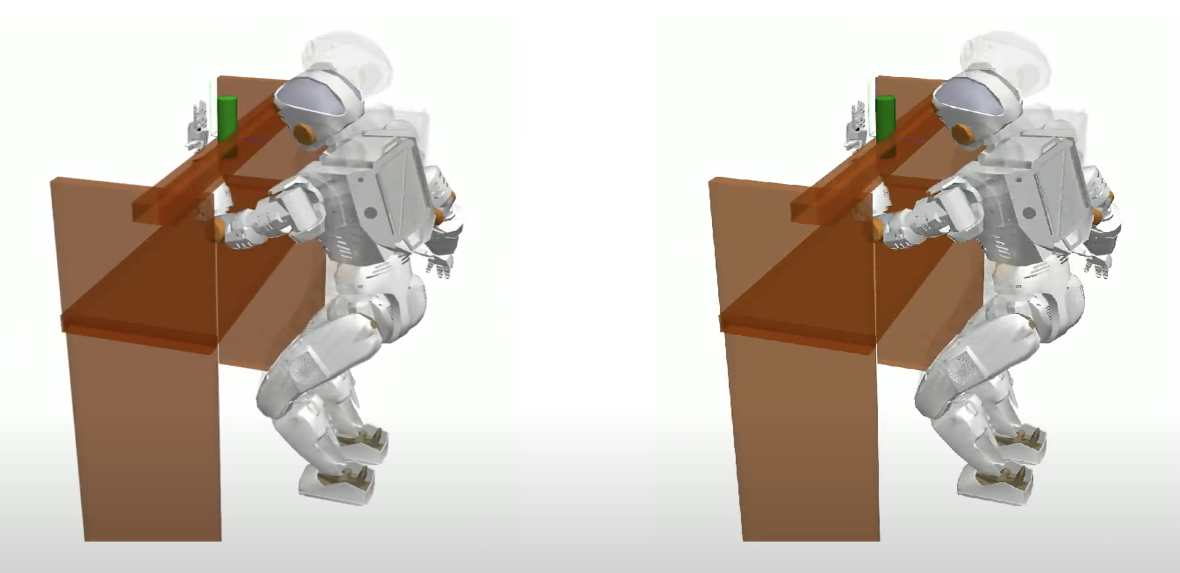
\includegraphics[scale=0.3]{images/motion-planning.png}\hfill
    \caption{Sampling based motion planning of NASA Valkyrie \cite{Vijayakumar}}\hfill
    \label{motion-planning}
\end{figure}

\begin{enumerate}
    \item \textit{Deterministic algorithms -} The deterministic algorithms are developed such that it computes the valid path everytime knowing almost
    all the variables of the environment. Methods such as \textit{cellular decomposition, Voronoi diagrams, visibility graphs, potential fields and Canny's algorithms}
    rely on
    mathematical construction of the environment with the obstacles and provide $\mathit{CS_{obs}}$. Although these algorithms are complete, the computation
    of high-dimensional space is expensive and the environments are always not deterministic.

    \item \textit{Sampling based algorithms -} These algorithms mostly approximate the connectivity of $\mathit{CS_{free}}$ through random sampling configurations
    from $\mathit{CS}$ and rejecting the configurations using boolean collision detection techniques. The main examples are  \textit{Probabilistic Maps and
    Rapidly-exploring Random Trees(RRT)} in combination with Voronoi diagrams promotes the obstacle avoidance configurations for a robot. The main advantage of
    sampling based algorithms are to handle the higher dimensional configuration space recovering a higher degree of completeness.

    \item \textit{Path optimization algorithms -} These algorithms provide optimization in terms of path planning and trajectory planning starting from a valid
    initial state to its goal position with the desired configurations. \textit{Greedy optimization} tries to directly connect the start configuration to 
    its goal state that generates a collision free shortest path by discretizing the path into \textit{n} closest goal configuration relative to previous 
    configuration.
\end{enumerate}

\subsubsection{Motion Planning in Humanoid robots}

\subsection{Kinematics Approach}
\subsection{Dynamics Approach}
\subsection{Optimal Control}

\section{Approaches in Humanoid Balance Control}
\subsection{Linear Inverse Pendulum Approach}
\subsection{Double Inverse Pendulum Approach}
\subsection{Cart Table Model}
\subsection{Spherical Inverse Pendulum Approach}

\section{Approaches in Posture Control and Motion Retargetting}
\subsection{Mansard's work}
\subsection{D. Gucci's work}
\subsection{Kumar Munirathinam's work}

